
\begin{document}
Jorge Torres\\
Universidad de Los Andes\\
Metodos Computacionales Taller 5\\
\vspace{1cm}

\begin{figure}[h!]
  \includegraphics[scale=0.5]{histogramax.png}
  \caption{Caso 1 Histograma en x }
\end{figure}
Podemos observar que la temperatura de mayor variacion son las condiciones de frontera periodicas, las condiciones fijas convergen a las temperaturas de las paredes del cubo.\\

\newpage
\begin{figure}[h!]
  \includegraphics[scale=0.5]{histogramay.png}
  \caption{Caso 2 Histograma en y }
\end{figure}

En el caso podemos observar que al haber un aumento constante de temperatura el promedio de todos los caso de frontera tambien aumentan , siendo mayor en las condiciones de frontera abiertas. Esto se debe a la fuente de calor constante.\\ 

\newpage
\begin{figure}[h!]
  \includegraphics[scale=0.5]{histogramar.png}
  \caption{Caso 3 Histograma en r }
\end{figure}

\newpage
\begin{figure}[h!]
  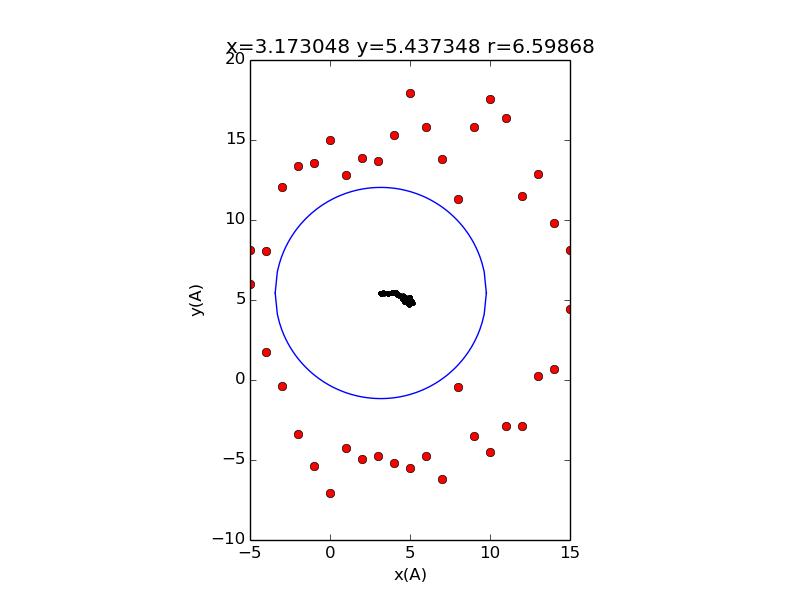
\includegraphics[scale=0.5]{radio_de_poro.png}
  \caption{Distancia del poro y los datos }
\end{figure}

\vspace{1cm}

\newpage
\begin{figure}[h!]
  \includegraphics[scale=0.35]{C1_ab_T0.png}
  \includegraphics[scale=0.35]{C1_ab_T2.png}
  \includegraphics[scale=0.35]{C1_ab_T3.png}
  \caption{Caso Abierto Temperatura}
\end{figure}
Vemos graficamente como los valores de la temperatura aumenta con respecto al tiempo y al estar la placa de mayor temperatura cerca al borde izquierdo esta sera la que aumenta mas rapdio su temperatura (con respecto a los otros bordes).
\vspace{1cm}

\newpage

\begin{figure}[h!]
  \includegraphics[scale=0.35]{C1_fi_T0.png}
  \includegraphics[scale=0.35]{C1_fi_T2.png}
  \includegraphics[scale=0.35]{C1_fi_T3.png}
  \caption{Caso Fijas Temperatura promedio}
\end{figure}
La escala esta mal selecionada por lo cual no se pueden osbervar claramente como las anterioras, toda la placa es con temperatura uniforme, por lo cual las diferencias no son significativas(observar la escala de los colores)
\vspace{1cm}




\end{figure}
\end{document}